\subsection*{Figure S3 · Calibrating the sparsity threshold (E12)}
\addcontentsline{toc}{subsection}{Figure S3 · Calibrating the sparsity threshold (E12)}
\noindent\emph{Referred to from the main paper, \S7.8.}

\begin{figure}[htbp]
\centering
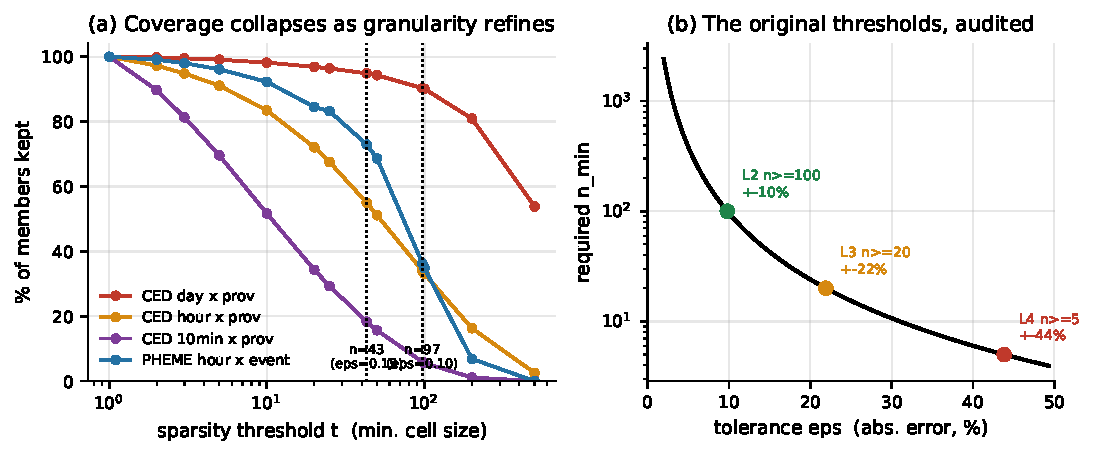
\includegraphics[width=0.88\columnwidth]{fig6_threshold_calibration.pdf}
\caption{Calibrating the sparsity threshold (E12). (a) Members kept by
qualified cells as the threshold grows: the same 1.09M posts lose coverage
rapidly as time granularity refines. (b) The required sample size
$n_{\min}(\varepsilon)\approx0.96/\varepsilon^2$ with the original D8
thresholds audited on the curve: L2 ${\ge}$100 sound, L3 ${\ge}$20 loose, L4
${\ge}$5 meaningless.}
\label{sfig:threshold}
\end{figure}
